% !TeX root = main-presentation.tex
\usepackage{figures/tikzit}
\usepackage{graphicx}
\usepackage{amssymb}
\usepackage{xparse}

\input{macros/sets}
\input{macros/category}
\input{macros/circuits}
\input{macros/streams}

\graphicspath{{./imgs/}}

\usetheme[
  background=light,
  numbering=counter,
  block=fill,
  %sectionpage=simple
]{metropolis}

\input{figures/circuits.tikzstyles}
\input{figures/circuits.tikzdefs}

% FiraFonts
\usepackage[sfdefault]{FiraSans}
\usepackage{FiraMono}
% Use thinner fonts
\makeatletter
\def\bfseries@sf{medium}
\def\mdseries@sf{l}
\makeatother

\definecolor{backg}{RGB}{9,72,61}
\definecolor{accent}{RGB}{0,150,136}

\definecolor{dracback}{RGB}{40, 42, 54}
\definecolor{dracfore}{RGB}{248, 248, 242}
\definecolor{dractitle}{RGB}{56, 58, 89}
\definecolor{dracblock}{RGB}{98, 114, 164}
\definecolor{draccent}{RGB}{255, 121, 198}

\setbeamercolor{normal text}{bg=dracfore}
\setbeamercolor{frametitle}{bg=dractitle, fg=dracfore}
\setbeamercolor{title separator}{fg=draccent}
\setbeamercolor{progress bar}{fg=draccent, bg=draccent}
\setbeamercolor{block title}{fg=dracfore, bg=dracblock}
\setbeamercolor{alerted text}{fg=draccent}

\newcommand{\wait}{\iftoggle{static}{}{\pause}}

\newtheorem{proposition}{Proposition}

\title{Fully abstract categorical semantics for digital circuits}
\author{\texorpdfstring{\large\textbf{George Kaye}, David Sprunger and Dan Ghica \\ \normalsize University of Birmingham}{George Kaye}}
\institute{ACT 2022}
\date{20 July 2022}

\begin{document}
    \maketitle

    % !TeX root = ../main-presentation.tex
\begin{frame}
    \frametitle{Joint work with...}

    \begin{minipage}{0.49\textwidth}
        \centering
        
\includegraphics[width=0.5\textwidth]{imgs/sprunger}
        
        David Sprunger
    \end{minipage}
    \begin{minipage}{0.49\textwidth}
        \centering
        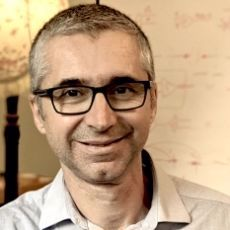
\includegraphics[width=0.5\textwidth]{imgs/ghica}
        
        Dan Ghica
    \end{minipage}

\end{frame}

\begin{frame}
    \frametitle{Introduction}
    
    Digital circuits are everywhere!

    \pause

    How do we reason with them?

\end{frame}

\begin{frame}
    \frametitle{Introduction}

    Generally by \alert{simulation}.

    \pause

    Reasoning in \alert{software} is more \alert{reduction-based}:

    \[
        (\lambda x.\lambda y.\, x + y) \, 2 \, 5 
        \pause\
        \rightsquigarrow_{\beta}
        \
        (\lambda y. 2 + y) \, 5 
        \pause\
        \rightsquigarrow_{\beta}
        \
        2 + 5 
        \pause\
        \rightsquigarrow_{\eta}
        \
        7
    \]
    
    \pause
    We want something similar for hardware.
\end{frame}
    \section{Syntax}

\begin{frame}
    \frametitle{Combinational circuit components}

    \renewcommand{\arraystretch}{1.25}

    \vspace{1em}
    \wait
    \begin{minipage}{0.33\textwidth}
        \centering

        \alert{Values}

        \vspace{1em}

        \begin{tabular}{rl}
            \tikzfig{circuits/components/values/false} &
            false \\
            \tikzfig{circuits/components/values/true} &
            true \\
            \wait
            \tikzfig{strings/structure/monoid/init} &
            disconnected \\
            \tikzfig{strings/structure/monoid/init-white} &
            short circuit \\
        \end{tabular}

        \vspace{1em}
        {\small\emph{(Belnap's four valued logic)}}
    \end{minipage}
    \wait
    \begin{minipage}{0.33\textwidth}
        \centering
        \alert{Gates}

        \renewcommand{\arraystretch}{2}

        \vspace{1em}
    
        \begin{tabular}{rl}
            \tikzfig{circuits/components/gates/and} &
            AND gate \\
            \tikzfig{circuits/components/gates/or} &
            OR gate \\
            \tikzfig{circuits/components/gates/not} &
            NOT gate \\
        \end{tabular}
    \end{minipage}
    \wait
    \begin{minipage}{0.32\textwidth}
        \centering
        \alert{Structure}

        \vspace{1em}
        
        \renewcommand{\arraystretch}{1.75}
        \begin{tabular}{cl}
            \wait
            \tikzfig{strings/category/identity} &
            identity \\
            \tikzfig{strings/symmetric/symmetry} &
            symmetry \\
            \wait
            \tikzfig{strings/structure/comonoid/copy} &
            fork \\
            \wait
            \tikzfig{strings/structure/monoid/merge} &
            join \\
            \wait
            \tikzfig{strings/structure/comonoid/discard} &
            stub \\
        \end{tabular}
    \end{minipage}

    \vspace{0.5em}

    \wait
    \begin{center}
        \alert{Light} circuits \(\tikzfig{circuits/components/circuits/f-comb}\) only contain gates and structure.
    \end{center}
\end{frame}

\begin{frame}
    \frametitle{Sequential circuit components}

    \wait

    \begin{minipage}{0.33\textwidth}
        \centering
        \alert{Delay}

        \[
            \tikzfig{circuits/components/delay}    
        \]
    \end{minipage}
    \wait
    \begin{minipage}{0.66\textwidth}
        \centering
        \alert{Feedback}

        \[
            \tikzfig{circuits/components/circuits/f-seq-2-2}
            \,\,\Rightarrow\,\,    
            \tikzfig{circuits/components/circuits/f-seq-traced}
        \]
    \end{minipage}

    \vspace{1em}

    \wait

    \begin{center}
        \alert{Dark} circuits \(\tikzfig{circuits/components/circuits/f-seq}\) may contain delay or feedback.        
    \end{center}

\end{frame}

\begin{frame}
    \frametitle{Circuit morphisms}

    Morphisms in a \alert{freely generated symmetric traced monoidal category}

    \[
        \tikzfig{circuits/examples/simple-and}  
    \]

\end{frame}

    \section{Semantics}

\begin{frame}
    \frametitle{Interpretation}

    Values are interpreted in a \alert{lattice} \(\values\):

    \begin{minipage}{0.49\textwidth}
        \[
            \tikzfig{circuits/a4}
        \]
    \end{minipage}
    \begin{minipage}{0.49\textwidth}
        \begin{align*}
            \tikzfig{circuits/components/values/false} 
            \,&\mapsto\, 0 \\
            \tikzfig{circuits/components/values/true} 
            \,&\mapsto\, 1 \\
            \tikzfig{strings/structure/monoid/init} 
            \,&\mapsto\, \bot \\
            \tikzfig{strings/structure/monoid/init-white} 
            \,&\mapsto\, \top \\
        \end{align*}
    \end{minipage}
\end{frame}

\begin{frame}
    \frametitle{Interpretation}

    \setlength{\tabcolsep}{1em}
    \renewcommand{\arraystretch}{2}

    \begin{center}
        \begin{tabular}{ll}
            \tikzfig{circuits/components/gates/gate} & \alert{monotone functions} \(\morph{\overline{g}}{\valuetuple{m}}{\values}\) \\ \pause
            \tikzfig{strings/structure/comonoid/copy} & \alert{copy} \(x \mapsto (x, x)\) \\ \pause
            \tikzfig{strings/structure/monoid/merge} & \alert{join in the lattice} \((x, y) \mapsto x \ljoin y\) \\ \pause
            \tikzfig{strings/structure/comonoid/discard} & \alert{discard} \(x \mapsto \bullet\)
        \end{tabular}
    \end{center}
\end{frame}

\begin{frame}
    \frametitle{Stream functions}

    The semantics of circuits is that of \alert{stream functions}.

    \pause

    A \alert{stream} \(\stream{\values}\) is an infinite sequence of values.
    
    \pause
    
    A \alert{stream function} \(\morph{f}{\stream{(\valuetuple{m})}}{\stream{(\valuetuple{n})}}\) consumes and produces streams.

    \pause

    For stream \(\sigma\), \(\sigma(i)\) is the \alert{\(i\)th element}.

\end{frame}

\begin{frame}
    \frametitle{Components as streams}

    \setlength{\tabcolsep}{1em}
    \renewcommand{\arraystretch}{2}

    \begin{center}
        \begin{tabular}{cll}
            \tikzfig{circuits/components/values/v} & \pause \(f(\bullet)(0) = v\) & \pause \(f(\bullet)(k+1) = \bot\) \\ \pause
            \tikzfig{circuits/components/gates/gate} & \pause \(f(\sigma)(k) = \overline{g}(\sigma(k))\) &  \\ \pause
            \tikzfig{circuits/components/delay} & \pause \(f(\sigma)(0) = \bot\) & \pause \(f(\sigma)(k+1) = \sigma(k)\)
        \end{tabular}
    \end{center}
    

\end{frame}

\begin{frame}
    \frametitle{Stream functions: example}

        \[
            \morph{f}{\stream{\values}}{\stream{\values}} := \circuittostream[\tikzfig{circuits/examples/simple-and}]{}
        \]

        \vspace{1em}

        \pause
        \[
            f(\sigma)(i) =
            \begin{cases}
                \pause 1 \land \sigma(0) & i = 0 \\
                \pause f(\sigma)(k) \land \sigma(k+1) & i = k+1
                
            \end{cases}
        \]
\end{frame}

\begin{frame}
    \frametitle{Stream functions}

    Not all stream functions correspond to sequential circuits...
    
\end{frame}

\begin{frame}
    \frametitle{Causal stream functions}

    Circuits cannot depend on \alert{future inputs}.

    \pause

    A stream function is \alert{causal} when the \(i\)th element of the output stream can only depend on the first \(i+1\) inputs.

    \pause

    \begin{center}
        \(
            \circuittostream[\tikzfig{circuits/examples/simple-and}]{}
        \)
        \qquad
        \(
            f(\sigma)(i) =
            \begin{cases}
                1 \land \sigma(0) & i = 0 \\
                f(\sigma)(k) \land \sigma(k+1) & i = k+1
                
            \end{cases}
        \)
    \end{center}
\end{frame}


\begin{frame}
    \frametitle{Monotone stream functions}

    Components in circuits are \alert{monotone}.

    A stream function is \alert{monotone} when computing each element of the output stream is a monotone function.

    \begin{center}
        \(
            \circuittostream[\tikzfig{circuits/examples/simple-and}]{}
        \)
        \qquad
        \(
            f(\sigma)(i) =
            \begin{cases}
                1 \land \sigma(0) & i = 0 \\
                f(\sigma)(k) \land \sigma(k+1) & i = k+1
                
            \end{cases}
        \)
    \end{center}

\end{frame}

\begin{frame}
    \frametitle{`Finite' stream functions}

    Circuits contain only a finite number of components.

    A stream function with \alert{finitely many stream derivatives} specifies finite behaviours given some inputs.

    \vspace{1em}

    \begin{center}
        \(
            \circuittostream[\tikzfig{circuits/examples/simple-and}]{}
        \)
        \qquad
        \(
            f(\sigma)(i) =
            \begin{cases}
                1 \land \sigma(0) & i = 0 \\
                f(\sigma)(k) \land \sigma(k+1) & i = k+1
                
            \end{cases}
        \)
        \pause

        \vspace{1.5em}

        \(
            f(0 \streamcons \sigma)(0) = 1 \land 0 = 0
        \)
        \pause

        \(
            f(0 \streamcons \sigma)(1) = f(0 \streamcons \sigma)(0) \land \sigma(0) = 0 \land \sigma(0) = 0
        \)\pause
        
        \(
            f(0 \streamcons \sigma)(2) = f(0 \streamcons \sigma)(1) \land \sigma(1) = 0 \land \sigma(1) = 0 = f(0 :: \sigma)(1)
        \)
    \end{center}

\end{frame}

\begin{frame}
    \frametitle{Stream functions for circuits}
    \begin{theorem}
        Every monotone causal stream function with finitely many stream derivatives corresponds to a class of sequential circuits. 
    \end{theorem}
\end{frame}
    % !TeX root = ../main-presentation.tex
\section{Equational reasoning}

\begin{frame}
    \frametitle{Equality of circuits}

    When are two circuits equal?

    \wait

    When they have the same \alert{beahviour}.

    \wait

    \[
        \tikzfig{circuits/examples/demorgan-lhs} 
        \quad
        \tikzfig{circuits/examples/demorgan-rhs} 
    \]

    When they have the same \alert{stream function}.

    \wait

    But reasoning with streams is a \alert{pain}.
    
\end{frame}

\begin{frame}
    \frametitle{Equational reasoning}

    We want to reason \alert{equationally}.

\end{frame}

\begin{frame}
    \frametitle{Productivity}


    A closed circuit is \alert{productive} if it can be reduced to an \alert{instant value} and a \alert{delayed subcircuit}.

    \[
        \tikzfig{circuits/components/circuits/f-seq-closed}
        \quad
        =
        \quad    
        \tikzfig{circuits/productivity/productive}
    \]

\end{frame}

\begin{frame}
    \frametitle{Combinational equations}
    \setlength{\jot}{2em}
    \wait
    \begin{center}
        \[
            \tikzfig{circuits/axioms/gate-lhs}
            \quad=\quad
            \tikzfig{circuits/axioms/gate-rhs}  
            \wait
            \qquad
            \tikzfig{strings/cartesian/naturality-copy-lhs}
            \quad=\quad
            \tikzfig{strings/cartesian/naturality-copy-rhs}
        \]\[
            \wait
            \tikzfig{circuits/axioms/join-lhs}
            \quad=\quad
            \tikzfig{circuits/axioms/join-rhs}
            \wait
            \qquad
            \tikzfig{strings/cartesian/naturality-discard-lhs}
            \quad=\quad
            \tikzfig{strings/cartesian/naturality-discard-rhs}
            \wait
        \]\[
            \tikzfig{strings/structure/comonoid/unitality-r-lhs}
            \quad=\quad
            \tikzfig{strings/structure/comonoid/unitality-r-rhs}
            \quad=\quad
            \tikzfig{strings/structure/comonoid/unitality-l-lhs}
        \]
    \end{center}

    \wait
    These reduce any \alert{closed combinational circuit} \(\tikzfig{circuits/components/circuits/f-comb-applied}\) to \(\tikzfig{circuits/components/values/ws}\).

\end{frame}

\begin{frame}
    \frametitle{Sequential equations}

    \[
        \tikzfig{circuits/axioms/disconnect-lhs}
        \quad=\quad
        \tikzfig{circuits/axioms/disconnect-rhs}    
        \qquad\wait
        \tikzfig{circuits/axioms/streaming-lhs-verbose}
        \quad=\quad
        \tikzfig{circuits/axioms/streaming-rhs}    
    \]
\end{frame}

\begin{frame}
    \frametitle{Non delay-guarded feedback}

    How de we deal with something like this?

    \[
        \tikzfig{circuits/productivity/trand}   
    \]

    \wait

    We need a way to eliminate \alert{non delay-guarded feedback}.

    \[
        \tikzfig{circuits/components/circuits/f-seq-traced}  
    \]

\end{frame}

\begin{frame}
    \frametitle{Non delay-guarded feedback}

    \wait

    Our gates are \alert{monotonic}, so they must have a \alert{least fixed point}...
    
    \[f^i(\bot) = f^{i+1}(\bot)\]

    \wait

    Because the value set \(\values\) is finite, we can always find this fixpoint!    
    
\end{frame}

\begin{frame}
    \frametitle{Non delay-guarded feedback}

    \(
        \tikzfig{circuits/a4}    
    \)
    \quad
    In \(\values\), the length of the longest chain is \alert{3}...

    \wait

    \[
        \tikzfig{circuits/components/circuits/f-seq-traced}
        \quad=\quad
        \tikzfig{circuits/instant-feedback/concrete-unfolding}
    \]
    

\end{frame}

\begin{frame}
    \frametitle{Eliminating `instant' feedback}

    \begin{center}
        \begin{minipage}{0.25\textwidth}
            \tikzfig{circuits/productivity/trand} 
            \quad\(=\)
        \end{minipage}
        \begin{minipage}{0.4\textwidth}
            \only<1>{
                \begin{center}
                    \tikzfig{circuits/examples/trand/step-1}
                \end{center}
            } 
            \only<2>{
                \begin{center}
                    \tikzfig{circuits/examples/trand/step-2}
                \end{center}
            }
            \only<3>{
                \begin{center}
                    \tikzfig{circuits/examples/trand/step-3}
                \end{center}
            }
            \only<4>{
                \begin{center}
                    \tikzfig{circuits/examples/trand/step-4}
                \end{center}
            }
        \end{minipage}
    \end{center}
\end{frame}

\begin{frame}
    \frametitle{Productivity}

    Now \alert{any} closed circuit is productive!


    \only<1>{
        \begin{center}
            \tikzfig{circuits/examples/reasoning/unfolding-dg/step-0}
        \end{center}
    }
    \only<2>{
        \begin{center}
            \tikzfig{circuits/examples/reasoning/unfolding-dg/step-0a}
        \end{center}
    }
    \only<3>{
        \begin{center}
            \tikzfig{circuits/examples/reasoning/unfolding-dg/step-1}
        \end{center}
    }
    \only<4>{
        \begin{center}
            \tikzfig{circuits/examples/reasoning/unfolding-dg/step-2}
        \end{center}
    }
    \only<5>{
        \begin{center}
            \tikzfig{circuits/examples/reasoning/unfolding-dg/step-3}
        \end{center}
    }
    \only<6>{
        \begin{center}
            \tikzfig{circuits/examples/reasoning/unfolding-dg/step-4}
        \end{center}
    }
    \only<7>{
        \begin{center}
            \tikzfig{circuits/examples/reasoning/unfolding-dg/step-5}
        \end{center}
    }
    \only<8>{
        \begin{center}
            \tikzfig{circuits/examples/reasoning/unfolding-dg/step-6}
        \end{center}
    }
    \only<9>{
        \begin{center}
            \tikzfig{circuits/examples/reasoning/unfolding-dg/step-7}
        \end{center}
    }
    \only<10>{
        \begin{center}
            \tikzfig{circuits/examples/reasoning/unfolding-dg/step-8}
        \end{center}
    }
    \only<11>{
        \begin{center}
            \tikzfig{circuits/examples/reasoning/unfolding-dg/step-9}
        \end{center}
    }
    \only<12>{
        \begin{center}
            \tikzfig{circuits/examples/reasoning/unfolding-dg/step-10}
        \end{center}
    }
    \only<13>{
        \begin{center}
            \tikzfig{circuits/examples/reasoning/unfolding-dg/step-11}
        \end{center}
    }
    \only<14>{
        \begin{center}
            \tikzfig{circuits/examples/reasoning/unfolding-dg/step-12}
        \end{center}
    }
    \only<15>{
        \begin{center}
            \tikzfig{circuits/examples/reasoning/unfolding-dg/step-13}
        \end{center}
    }
\end{frame}

\begin{frame}
    \frametitle{Open circuits}

    We still cannot necessarily translate between \alert{open} circuits with the same behaviour.

    \[
        \tikzfig{circuits/examples/demorgan-lhs} 
        \quad
        \tikzfig{circuits/examples/demorgan-rhs} 
    \]

    We need another equation.

\end{frame}

\begin{frame}
    \frametitle{Open circuits}

    When do these have the \alert{same stream}?

    \[
        \tikzfig{circuits/components/circuits/f-seq}
        \qquad
        \tikzfig{circuits/components/circuits/g-seq}
    \]

\end{frame}

\begin{frame}
    \frametitle{Open circuits}

    When do these have the \alert{same stream}?

    \[
        \tikzfig{circuits/components/circuits/f-seq}
        \quad=\quad
        \tikzfig{circuits/full-abstraction/global-delay-f}
        \qquad
        \tikzfig{circuits/components/circuits/g-seq}
        \quad=\quad
        \tikzfig{circuits/full-abstraction/global-delay-g}
    \]
    
    The outputs of \(\tikzfig{circuits/components/circuits/f-pre-trace-unlabelled}\) and \(\tikzfig{circuits/components/circuits/g-pre-trace-unlabelled}\) are the \alert{transition} and \alert{output}.

    \alert{Idea}: for all \alert{transitions}, check that \alert{outputs} are equal.

    \tiny{(cf. Mealy machine bisimulation)}
\end{frame}

\begin{frame}
    \frametitle{}

    Check the \alert{initial output}...

    \begin{center}
        

    \end{center}
    

\end{frame}
\end{document}
